\documentclass[11pt,a4paper]{article}
\usepackage[utf8]{inputenc}
\usepackage[margin=2.5cm]{geometry}
\usepackage{amsmath,amssymb,amsthm,mathtools}
\usepackage{booktabs,enumitem,tabularx,array}
\usepackage[expansion=false]{microtype}
\usepackage{float}
\usepackage{tikz}
\usetikzlibrary{positioning,arrows.meta,calc}
\usepackage[colorlinks=true,linkcolor=blue!60!black,citecolor=blue!60!black,urlcolor=blue!60!black]{hyperref}
\renewcommand{\arraystretch}{1.25}
\newcolumntype{L}{>{\raggedright\arraybackslash}X}
\DeclareTextSymbolDefault{\textsection}{OMS}
\renewcommand{\labelitemi}{$\bullet$}
\linespread{1.06}
\setlength{\parskip}{0.35em}
\setlength{\emergencystretch}{8em}

\renewcommand{\qedsymbol}{$\blacksquare$}

\theoremstyle{plain}
\newtheorem{theorem}{Theorem}[section]
\newtheorem{lemma}[theorem]{Lemma}
\newtheorem{corollary}[theorem]{Corollary}
\newtheorem{proposition}[theorem]{Proposition}
\theoremstyle{definition}
\newtheorem{definition}[theorem]{Definition}
\newtheorem{remark}[theorem]{Remark}
\newtheorem{example}[theorem]{Example}

\newcommand{\R}{\mathbb R}
\newcommand{\Z}{\mathbb Z}
\newcommand{\N}{\mathbb N}
\newcommand{\AM}{A_M}
\newcommand{\kerZ}{\ker_{\Z}\!A_M}
\newcommand{\kerR}{\ker_{\R}\!A_M}
\newcommand{\sq}{L_{\square}}
\newcommand{\bs}{\mathcal B}
\newcommand{\sgn}{\operatorname{sgn}}
\newcommand{\rank}{\operatorname{rank}}
\newcommand{\cl}{\operatorname{cl}}
\newcommand{\ind}{\mathbf 1}
\newcommand{\colex}{<_{\mathrm{colex}}}
\newcommand{\LM}{Laso\'n--Micha\l{}ek}

\title{A Square Basis Theorem for Matroids}
\author{Youngsu Kim}
\date{}

\begin{document}
\maketitle

\begin{abstract}
\noindent White's conjecture asserts that the toric ideal of every matroid is generated by symmetric exchange binomials, equivalently, that the exchange moves form a Markov basis; it fails in general. We prove that a lattice version holds for every matroid of rank at least one: the exponent vectors of the symmetric exchange binomials, the \emph{square relations} $e_{B+i}-e_{B+j}-e_{B'+i}+e_{B'+j}$, always contain a $\Z$-basis of the integer kernel $\kerZ$ of the basis incidence matrix $\AM$. Equivalently, over any field the toric ideal $I_M$ becomes, after inverting the variables, a complete intersection of $\operatorname{codim} I_M$ symmetric exchange binomials. The proof is constructive and combinatorial, and it uses no computer calculation. It combines a direct-sum decomposition, an exact sequence for single-element deletion, and a connectivity property of the circuits through a fixed element of a matroid, which is closely related to Lehman's theorem. For uniform matroids we give an explicit unitriangular square basis. As an application, we characterize when two real matrices differ by an invertible row transformation and an invertible column scaling. The criterion consists of square conditions on the signs and absolute values of their Pl\"ucker ratios, one for each element of a square basis. The sign conditions require this basis to be a $\Z$-basis, not merely an $\R$-basis.

\vspace{1.2em}\noindent\textbf{Keywords.} matroid, toric ideal, basis exchange, lattice basis, White's conjecture, Pl\"ucker coordinates

\smallskip\noindent\textbf{Mathematics Subject Classification.} 05B35, 13F65, 14M25
\end{abstract}

%====================================================================
\section{Introduction}\label{sec:intro}
White conjectured that the toric ideal $I_M$ of every matroid $M$ is generated by the quadratic binomials coming from symmetric basis exchange~\cite{W80}. The conjecture is known for matroids of rank at most $3$~\cite{Ka10}, graphic matroids~\cite{Bl08}, lattice path matroids~\cite{Sc11}, sparse paving matroids~\cite{Bo13}, paving matroids~\cite{YY25}, and strongly base orderable matroids~\cite{LM14}. For every matroid it holds up to saturation by the irrelevant ideal~\cite{LM14}, and for fixed rank it holds in high degree~\cite{La21}. It is preserved under adding or removing a single basis~\cite{HMW25}, and Gr\"obner bases were computed for all but two matroids on at most $7$ elements~\cite{HHKS20}. For regular and split matroids, the exchange distance between pairs of bases has also been studied~\cite{BMS24,BS24}. In 2026 Larson reported a counterexample to White's conjecture~\cite{Lar26}, and it was shown that matroids with a Fano or dual Fano minor have no quadratic Gr\"obner basis~\cite{BCLLM26,DFMR26}.

In the terminology of algebraic statistics~\cite{DS98}, White's conjecture asserts that the exchange moves form a \emph{Markov basis} of the lattice of $I_M$, and this fails in general. A different requirement, at the level of the lattice, is that the set of moves contain a \emph{lattice basis}, that is, a $\Z$-basis of the same lattice. We prove that this requirement holds for every matroid of rank at least $1$ (Theorem~\ref{thm:main}). The statement concerns the lattice of $I_M$, not generators of $I_M$ itself, so it is compatible with all of the results above (Remarks~\ref{rem:markov} and~\ref{rem:white}).

Let $M$ be a matroid of rank $k$ on $[n]=\{1,\dots,n\}$ with set of bases $\bs$, and let $N=|\bs|$. The \emph{basis incidence matrix} $\AM\in\{0,1\}^{n\times N}$ has the indicator vector $\ind_I$ of the basis $I$ as its column indexed by $I$. Its integer kernel
\[
\kerZ=\{u\in\Z^{\bs}:\AM u=0\}
\]
is a free abelian group of rank $N-\rank\AM$. It is the lattice of the toric ideal $I_M$ of $M$, the kernel of the map $y_I\mapsto\prod_{i\in I}x_i$~\cite{W77,St96}.

Basis exchange produces natural elements of this lattice. Let $i\ne j$, and let $B\ne B'$ be $(k-1)$-sets with $i,j\notin B\cup B'$. If $B+i$, $B+j$, $B'+i$, $B'+j$ are all bases, then $\ind_{B+i}-\ind_{B+j}=e_i-e_j=\ind_{B'+i}-\ind_{B'+j}$ in $\Z^n$. Hence, writing $e_I$ for the standard basis vector of $\Z^{\bs}$ indexed by $I\in\bs$, we have
\[
z_{i,j;B,B'}=e_{B+i}-e_{B+j}-e_{B'+i}+e_{B'+j}\in\kerZ .
\]
We call $z_{i,j;B,B'}$ a \emph{square relation}. The square relations are exactly the exponent vectors of the symmetric exchange binomials $y_{B_1}y_{B_2}-y_{B_1-a+b}\,y_{B_2-b+a}$ that appear in White's conjecture~\cite{W80} (Lemma~\ref{lem:sym}).

\begin{theorem}[Square Basis Theorem]\label{thm:main}
For every matroid $M$ of rank at least $1$, the lattice $\kerZ$ has a $\Z$-basis consisting of $N-\rank\AM$ square relations.
\end{theorem}

The rank condition is necessary: if $\rank M=0$, then $\kerZ=\Z$ but there are no squares. Figure~\ref{fig:u24} shows the smallest nontrivial uniform example.

\begin{figure}[H]
\centering
\newcommand{\octa}[3]{%
\begin{tikzpicture}[scale=0.95,v/.style={circle,fill=black,inner sep=1.1pt},lab/.style={font=\footnotesize}]
\coordinate (T) at (0,1.75);  \coordinate (D) at (0,-1.75);
\coordinate (L) at (-1.45,0); \coordinate (R) at (1.45,0);
\coordinate (K) at (0.55,0.42); \coordinate (F) at (-0.55,-0.42);
#1
\draw[gray!60,dashed] (T)--(K) (D)--(K) (L)--(K) (R)--(K);
\draw (T)--(L) (T)--(R) (T)--(F) (D)--(L) (D)--(R) (D)--(F) (L)--(F) (F)--(R);
#2
\foreach \p in {T,D,L,R,K,F} \node[v] at (\p) {};
\node[lab,above] at (T) {$12$}; \node[lab,below] at (D) {$34$};
\node[lab,left] at (L) {$24$}; \node[lab,right] at (R) {$13$};
\node[lab,above right=-1pt] at (K) {$14$}; \node[lab,below left=-1pt] at (F) {$23$};
\node[font=\small,align=center] at (0,-2.55) {#3};
\end{tikzpicture}}
\octa{\fill[blue!20] (L)--(K)--(R)--(F)--cycle;}{\draw[blue!70!black,very thick] (L)--(F)--(R); \draw[blue!70!black,very thick,dashed] (R)--(K)--(L);}{$z_1=e_{13}-e_{14}+e_{24}-e_{23}$}\hfill
\octa{\fill[red!18] (T)--(K)--(D)--(F)--cycle;}{\draw[red!70!black,very thick] (T)--(F)--(D); \draw[red!70!black,very thick,dashed] (D)--(K)--(T);}{$z_2=e_{12}-e_{14}+e_{34}-e_{23}$}\hfill
\octa{\fill[green!20] (T)--(R)--(D)--(L)--cycle;}{\draw[green!40!black,very thick] (T)--(R)--(D)--(L)--cycle;}{$z_3=e_{12}-e_{13}+e_{34}-e_{24}$}
\caption{The base polytope of $U_{2,4}$ is an octahedron whose vertices are the six bases $I\subset[4]$, $|I|=2$; antipodal vertices are complementary sets. Up to sign, its three equatorial squares are exactly the square relations (signs alternate around each square). Here $\rank\kerZ=6-4=2$ and $z_1=z_2-z_3$, so any two of the three squares form a $\Z$-basis of $\kerZ$.}
\label{fig:u24}
\end{figure}

\medskip\noindent\textbf{Why a basis matters.} Theorem~\ref{thm:main} strengthens two known facts about matroids of rank at least $1$. Over $\R$, the squares span $\kerR$, as also follows from Theorem~\ref{thm:sat} below, so some $N-\rank\AM$ squares form an $\R$-basis; but an $\R$-basis of a lattice need not generate it. Over $\Z$, the squares generate $\kerZ$, which follows from the \LM{} theorem~\cite{LM14} (Proposition~\ref{prop:lattice}); but a generating set of a free abelian group need not contain a basis (for example, $\{2,3\}$ generates $\Z$, but no subset of it is a basis of $\Z$). Theorem~\ref{thm:main} gives both properties at once: a set of squares that generates $\kerZ$ over $\Z$ and has the least possible size. This has the following consequences.

\begin{enumerate}[label=(\roman*),leftmargin=2em,itemsep=2pt]
\item \emph{Toric ideals.} Let $c=N-\rank\AM$, which is the codimension of $I_M$. Theorem~\ref{thm:main} is equivalent to the existence of $c$ symmetric exchange binomials $f_1,\dots,f_c$ with
\[
I_M\,K[y^{\pm1}]=(f_1,\dots,f_c)\,K[y^{\pm1}],\qquad I_M=(f_1,\dots,f_c):\Big(\prod_{I\in\bs}y_I\Big)^{\infty}
\]
over any field $K$ (Corollary~\ref{cor:toric}). By Krull's height theorem, neither equation can hold with fewer than $c$ generators. Geometrically, the part of the toric variety of $M$ that lies in the torus $(K^\times)^{\bs}$ is a complete intersection of $c$ symmetric exchange quadrics. By contrast, $I_M$ itself is rarely a complete intersection: if $M$ has no loops or coloops and $c\ge1$, this happens only for three matroids on four elements~\cite{GR15}.
\item \emph{Local certificates.} Let $\Theta$ be any abelian group, for instance $\Z/2$ or $\R$. If a function $\chi:\bs\to\Theta$ satisfies the square condition $\chi(B+i)-\chi(B+j)-\chi(B'+i)+\chi(B'+j)=0$ for the $c$ squares of a square basis, then $\sum_I u_I\chi(I)=0$ for every $u\in\kerZ$, because $u\mapsto\sum_Iu_I\chi(I)$ is a homomorphism vanishing on a generating set. For a torsion group such as $\Z/2$, an $\R$-basis of squares does not suffice for this in general, since it may generate a proper sublattice of finite index (Remark~\ref{rem:index}), and a generating set of squares that is not a basis has more than $c$ elements. The cases $\Theta=\Z/2$ and $\Theta=\R$ together give a criterion for two real matrices to differ by an invertible row transformation and an invertible column scaling (\S\ref{sec:criterion}).
\end{enumerate}


\medskip\noindent\textbf{Outline of the proof.} The proof does not use the \LM{} theorem; its structure is summarized in Figure~\ref{fig:map}. First, direct sums reduce the problem to connected matroids (\S\ref{sec:dsum}). Next, let $M$ be a connected matroid and $v$ an element with $M\setminus v$ connected. An exact sequence $0\to\ker_\Z A_{M\setminus v}\to\kerZ\to\Gamma\to0$ allows us to lift a square basis of $M\setminus v$ to $M$, provided that a certain graph on $[n]-v$ is connected (\S\ref{sec:conn}). This graph is connected exactly when the cocircuits of $M$ through $v$, that is, the circuits of $M^*$ through $v$, link all other elements (Proposition~\ref{prop:phi}). In \S\ref{sec:phiproof} we prove that in a connected matroid $P$ the circuits through $v$ link all other elements whenever $P/v$ is connected (Theorem~\ref{thm:phi}); for $P=M^*$, since $P/v=(M\setminus v)^*$, this hypothesis says exactly that $M\setminus v$ is connected. Finally, by Tutte's theorem~\cite[Section~4.3]{Ox11}, $M\setminus v$ or $M/v$ is connected; if $M/v$ is connected, then $M^*\setminus v=(M/v)^*$ is connected, and duality (Lemma~\ref{lem:dual}) reduces this case to the previous one applied to $M^*$. This completes the induction. For uniform matroids an explicit basis is given in \S\ref{sec:uniform}.

\begin{figure}[H]
\centering
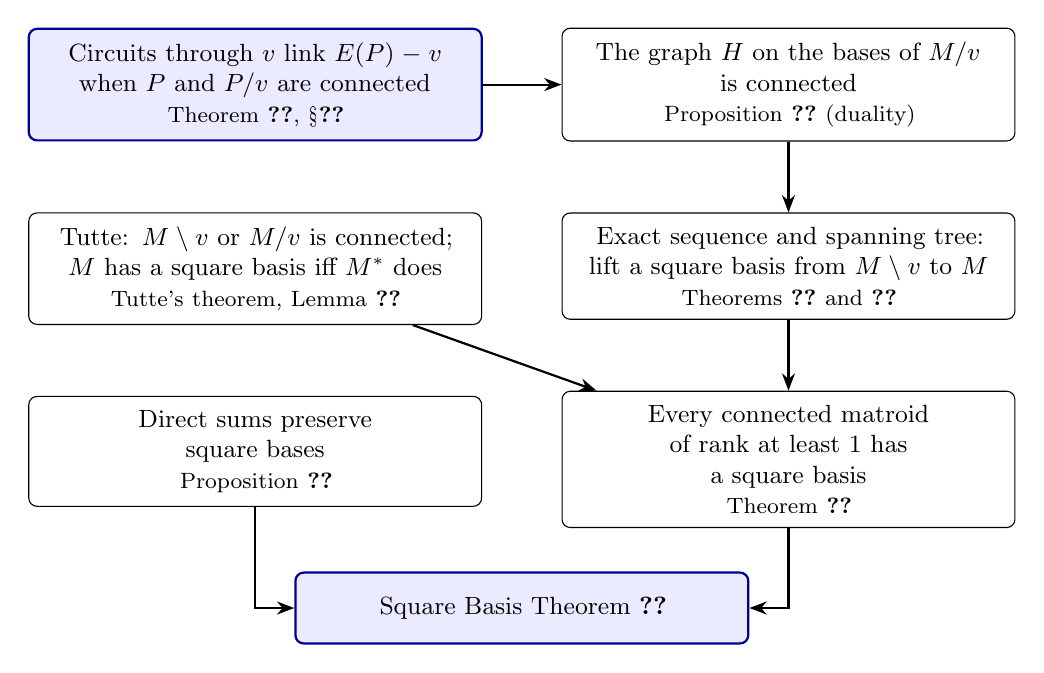
\begin{tikzpicture}[
  box/.style={draw,rounded corners=3pt,align=center,font=\small,inner sep=5pt,text width=5.4cm,minimum height=1.35cm},
  key/.style={box,fill=blue!8,draw=blue!60!black,thick},
  arr/.style={-{Stealth[length=2.2mm]},thick}]
\node[key] (phi) {Circuits through $v$ link $E(P)-v$\\ when $P$ and $P/v$ are connected\\ \footnotesize Theorem~\ref{thm:phi}, \S\ref{sec:phiproof}};
\node[box,right=1.0cm of phi] (H) {The graph $H$ on the bases of $M/v$\\ is connected\\ \footnotesize Proposition~\ref{prop:phi} (duality)};
\node[box,below=0.9cm of H] (lift) {Exact sequence and spanning tree:\\ lift a square basis from $M\setminus v$ to $M$\\ \footnotesize Theorems~\ref{thm:exact} and \ref{thm:tree}};
\node[box,below=0.9cm of phi] (tutte) {Tutte: $M\setminus v$ or $M/v$ is connected;\\ $M$ has a square basis iff $M^*$ does\\ \footnotesize Tutte's theorem, Lemma~\ref{lem:dual}};
\node[box,below=0.9cm of lift] (conn) {Every connected matroid\\ of rank at least $1$ has\\ a square basis\\ \footnotesize Theorem~\ref{thm:cond}};
\node[box,below=0.9cm of tutte] (dsum) {Direct sums preserve\\ square bases\\ \footnotesize Proposition~\ref{prop:dsum}};
\node[key,minimum height=0.9cm] (main) at ($(dsum.south)!0.5!(conn.south)+(0,-1.15)$) {Square Basis Theorem~\ref{thm:main}};
\draw[arr] (phi)--(H);
\draw[arr] (H)--(lift);
\draw[arr] (lift)--(conn);
\draw[arr] (tutte)--(conn);
\draw[arr] (conn.south) |- ($(main.east)+(0,0)$);
\draw[arr] (dsum.south) |- ($(main.west)+(0,0)$);
\end{tikzpicture}
\caption{Structure of the proof. The shaded box at the upper left is the main matroid-theoretic step. Section~\ref{sec:phiproof} gives a self-contained proof, and Remark~\ref{rem:lehman} derives it from Lehman's theorem.}
\label{fig:map}
\end{figure}

\medskip\noindent\textbf{Organization.} Section~\ref{sec:prelim} fixes notation. Sections~\ref{sec:dsum}--\ref{sec:phiproof} prove Theorem~\ref{thm:main}. Section~\ref{sec:uniform} treats uniform matroids. Section~\ref{sec:apps} gives the consequences for toric ideals and the application to invertible column scaling, and Section~\ref{sec:caveats} discusses the relation to the \LM{} theorem and open problems.

%====================================================================
\section{Preliminaries}\label{sec:prelim}
We use the matroid terminology of Oxley~\cite{Ox11}. For a set $I$ and an element $a$ we write $I+a=I\cup\{a\}$ and $I-a=I\setminus\{a\}$. Since every basis has size $k$, $\AM^{T}\ind_n=k\,\ind_{\bs}$; hence every $u\in\kerZ$ has coordinate sum $0$ when $k\ge1$. Over a field $K$, write $K[y]=K[y_I:I\in\bs]$. The toric ideal $I_M\subseteq K[y]$ is the kernel of the homomorphism $K[y]\to K[x_1,\dots,x_n]$, $y_I\mapsto\prod_{i\in I}x_i$, and by~\cite{St96}
\[
I_M=\big(y^{u^+}-y^{u^-}:u\in\kerZ\big),
\]
where $u=u^+-u^-$ with $u^\pm\in\N^{\bs}$ of disjoint supports and $y^w=\prod_Iy_I^{w_I}$. The Krull dimension of $K[y]/I_M$ is $\rank\AM$, so $I_M$ has height $N-\rank\AM$.

\begin{definition}\label{def:square}
For distinct $i,j\in[n]$ and distinct $(k-1)$-subsets $B,B'$ with $i,j\notin B\cup B'$ such that $B+i,B+j,B'+i,B'+j$ are bases, the vector $z_{i,j;B,B'}=e_{B+i}-e_{B+j}-e_{B'+i}+e_{B'+j}\in\Z^{\bs}$ is a \emph{square relation}, or \emph{square}. We write $\sq(M)$ for the sublattice of $\Z^{\bs}$ generated by the squares, and we say that $M$ \emph{has a square basis} if $\kerZ$ has a $\Z$-basis consisting of squares.
\end{definition}
Since the four indicator vectors satisfy $\ind_{B+i}-\ind_{B+j}-\ind_{B'+i}+\ind_{B'+j}=0$, we always have $\sq(M)\subseteq\kerZ$. A \emph{symmetric exchange} consists of bases $B_1,B_2$ and elements $a\in B_1\setminus B_2$, $b\in B_2\setminus B_1$ such that $B_1-a+b$ and $B_2-b+a$ are bases; its binomial is $y_{B_1}y_{B_2}-y_{B_1-a+b}\,y_{B_2-b+a}$.

\begin{lemma}\label{lem:sym}
The squares are exactly the exponent vectors of the nonzero symmetric exchange binomials.
\end{lemma}
\begin{proof}
Given a square, put $B_1=B+i$, $B_2=B'+j$, $a=i$, $b=j$. Then $B_1-a+b=B+j$ and $B_2-b+a=B'+i$, and $i,j\notin B\cup B'$ is equivalent to $a\in B_1\setminus B_2$, $b\in B_2\setminus B_1$. Conversely, given a symmetric exchange, set $B=B_1-a$, $B'=B_2-b$, $i=a$, $j=b$; the binomial is zero exactly when $B=B'$.
\end{proof}

\begin{proposition}[Boundary cases]\label{prop:edge}
\begin{enumerate}[label=(\alph*),itemsep=1pt]
\item If $\rank M=0$, then $\bs=\{\varnothing\}$ and $\kerZ=\Z$, but there are no squares.
\item Deleting a loop changes neither $\kerZ$ nor the set of squares.
\item If $M=M'\oplus\{c\}$ with $c$ a coloop and $\rank M'\ge1$, then $I'\mapsto I'+c$ induces an isomorphism $\ker_\Z A_{M'}\cong\kerZ$ that maps squares onto squares. If $\rank M'=0$, then $\kerZ=0$.
\end{enumerate}
\end{proposition}
\begin{proof}
(a) and (b) are immediate. (c) The row of $\AM$ indexed by $c$ is the all-ones vector, and the condition $\sum f=0$ it imposes already follows from the rows of $M'$ when $\rank M'\ge1$. It remains to see that $c\in B\cap B'$ for every square $z_{i,j;B,B'}$ of $M$. If $c\notin B\cup B'$, then $B+i$ and $B+j$ both contain the coloop $c$, which forces $i=c=j$, contradicting $i\ne j$. If $c\in B\setminus B'$, then $c\in B'+i$ forces $i=c\in B$, a contradiction; the case $c\in B'\setminus B$ is symmetric.
\end{proof}

\begin{lemma}[Duality]\label{lem:dual}
If $1\le k\le n-1$, then $e_I\mapsto e_{[n]\setminus I}$ induces an isomorphism $\kerZ\to\ker_\Z A_{M^*}$ that maps the square $z_{i,j;B,B'}$ to $-z_{i,j;C,C'}$, where $C=[n]\setminus(B+i+j)$ and $C'=[n]\setminus(B'+i+j)$. Hence $M$ has a square basis if and only if $M^*$ does.
\end{lemma}
\begin{proof}
For $f\in\kerZ$ we have $\sum f=0$, and the condition from row $i$ of $A_{M^*}$ is $\sum_{I\not\ni i}f(I)=\sum f-(\AM f)_i=0$. The converse is the same argument applied to $M^{*}$, using $M^{**}=M$. For squares, $[n]\setminus(B+i)=C+j$, $[n]\setminus(B+j)=C+i$, and similarly for $B'$.
\end{proof}

%====================================================================
\section{Direct sums}\label{sec:dsum}
Let $M=M_1\oplus M_2$ with ground sets $E_1,E_2$. The bases of $M$ are the sets $I_1\sqcup I_2$ with $I_t\in\bs_t=\bs(M_t)$, so $\Z^{\bs}=V_1\otimes V_2$ with $V_t=\Z^{\bs_t}$. Write $N_t=|\bs_t|$, $\rho_t=\rank A_{M_t}$, $K_t=\ker_\Z A_{M_t}$, $k_t=\rank M_t$, and let $V_t^0\subseteq V_t$ be the sublattice of vectors with coordinate sum $0$.

\begin{proposition}\label{prop:dsum}
If $k_1,k_2\ge1$ and $M_1,M_2$ have square bases $\mathcal R_1,\mathcal R_2$, then $M_1\oplus M_2$ has a square basis.
\end{proposition}
\begin{proof}
\emph{Step 1 (the kernel).} For $f\in V_1\otimes V_2$ let $\operatorname{row}(f)(I_1)=\sum_{I_2}f(I_1,I_2)$ and $\operatorname{col}(f)(I_2)=\sum_{I_1}f(I_1,I_2)$. The rows of $\AM$ indexed by $E_1$ give $A_{M_1}\operatorname{row}(f)$ and those indexed by $E_2$ give $A_{M_2}\operatorname{col}(f)$, so
\[
\kerZ=\{f:\operatorname{row}(f)\in K_1,\ \operatorname{col}(f)\in K_2\},
\]
and $K_t\subseteq V_t^0$ because $k_t\ge1$.

\emph{Step 2 (decomposition).} Fix $I_1^0\in\bs_1$ and $I_2^0\in\bs_2$. Then
\[
\kerZ=K_1\otimes e_{I_2^0}\ \oplus\ e_{I_1^0}\otimes K_2\ \oplus\ (V_1^0\otimes V_2^0).
\]
The first two summands carry the kernels of the two factors, and the third consists of the interaction terms. Each summand lies in $\kerZ$ by Step 1; note that $V_1^0\otimes V_2^0$ is exactly the set of $f$ with $\operatorname{row}(f)=0$ and $\operatorname{col}(f)=0$. For $f\in\kerZ$ put $f'=f-\operatorname{row}(f)\otimes e_{I_2^0}-e_{I_1^0}\otimes\operatorname{col}(f)$; since $\sum\operatorname{row}(f)=\sum\operatorname{col}(f)=0$, we get $\operatorname{row}(f')=\operatorname{col}(f')=0$. Applying $\operatorname{row}$ and $\operatorname{col}$ shows that the sum is direct.

\emph{Step 3 (a basis of $V_1^0/K_1$).} The lattice $\Lambda_1=A_{M_1}(V_1^0)$ is generated by the vectors $\ind_J-\ind_{J'}$ with $J,J'\in\bs_1$. Since the basis exchange graph is connected~\cite{Br69}, adjacent pairs suffice, and for $J=D+a$, $J'=D+b$ we get $e_a-e_b$. Let $G_1$ be the graph on $E_1$ with $a\sim b$ if $D+a,D+b\in\bs_1$ for some $D$, and let $F_1$ be a spanning forest of $G_1$. The vectors $e_a-e_b$, $\{a,b\}\in F_1$, form a $\Z$-basis of $\Lambda_1$. Since $A_{M_1}(V_1)=\Lambda_1+\Z\ind_{J_0}$ for any $J_0\in\bs_1$ and $\ind_{J_0}$ has coordinate sum $k_1\neq0$, we have $|F_1|=\rank\Lambda_1=\rho_1-1$. For each edge $\{a,b\}\in F_1$ choose $D_{ab}$ with $D_{ab}+a,D_{ab}+b\in\bs_1$ and put $u_{ab}=e_{D_{ab}+a}-e_{D_{ab}+b}\in V_1^0$. Then $A_{M_1}u_{ab}=e_a-e_b$, and since $A_{M_1}$ induces an isomorphism $V_1^0/K_1\cong\Lambda_1$, the classes $\overline{u_{ab}}$ form a $\Z$-basis of $V_1^0/K_1$.

\emph{Step 4 (the basis).} The subgroup $K_1\otimes V_2=K_1\otimes e_{I_2^0}\oplus K_1\otimes V_2^0$ of $\kerZ$ has free quotient
\[
\kerZ/(K_1\otimes V_2)\cong e_{I_1^0}\otimes K_2\ \oplus\ (V_1^0/K_1)\otimes V_2^0 .
\]
Using the basis $\{e_I-e_{I_2^0}\}_{I\ne I_2^0}$ of $V_2^0$, we obtain the following $\Z$-basis of $\kerZ$:
\begin{enumerate}[label=(\arabic*),itemsep=1pt]
\item $w\otimes e_I$ for $w\in\mathcal R_1$, $I\in\bs_2$;
\item $e_{I_1^0}\otimes s$ for $s\in\mathcal R_2$;
\item $u_{ab}\otimes(e_I-e_{I_2^0})$ for $\{a,b\}\in F_1$, $I\in\bs_2\setminus\{I_2^0\}$.
\end{enumerate}
Their number is $N_1N_2-\rho_1-\rho_2+1=N_1N_2-\rank\AM$, since $\AM f=(A_{M_1}\operatorname{row}(f),\,A_{M_2}\operatorname{col}(f))$ and the pairs $(\operatorname{row}(f),\operatorname{col}(f))$, as $f$ ranges over $\Z^{\bs}$, are exactly the pairs with equal coordinate sums.

\emph{Step 5 (all are squares).} If $w=z_{i,j;D,D'}$, then $w\otimes e_I=z_{i,j;D\sqcup I,\,D'\sqcup I}$; family (2) is analogous. For (3), take $B=D_{ab}\sqcup I$, $B'=D_{ab}\sqcup I_2^0$, $i=a$, $j=b$: the four sets $(D_{ab}+a)\sqcup I$, $(D_{ab}+b)\sqcup I$, $(D_{ab}+a)\sqcup I_2^0$, $(D_{ab}+b)\sqcup I_2^0$ are bases, $a,b\notin B\cup B'$, $B\ne B'$, and the square is $u_{ab}\otimes(e_I-e_{I_2^0})$.
\end{proof}

%====================================================================
\section{Connected matroids}\label{sec:conn}
In this section $M$ is a connected matroid with $n\ge2$, so it has no loops or coloops and $1\le k\le n-1$. Fix $v\in[n]$ and put $X=[n]-v$, $M_{\mathrm d}=M\setminus v$ and $M_{\mathrm c}=M/v$. The bases of $M_{\mathrm d}$ are the bases of $M$ avoiding $v$, and the bases of $M_{\mathrm c}$ are the sets $J\subseteq X$ with $J+v\in\bs$. For a matroid $M_0$ let $\Lambda(M_0)$ be the lattice generated by the indicator vectors of its bases.

\begin{lemma}\label{lem:lat}
If $M_0$ is a connected matroid of rank $k\ge1$ on $Y$, then $\Lambda(M_0)=\{x\in\Z^Y:\sum x\in k\Z\}$. In particular $\rank A_{M_0}=|Y|$.
\end{lemma}
\begin{proof}
The inclusion $\subseteq$ is clear. For distinct $i,j\in Y$ there is a circuit $C\ni i,j$. Extend $C-j$ to a basis $I$; then $C$ is the fundamental circuit of $j$ with respect to $I$ and contains $i$, so $I-i+j$ is a basis and $e_j-e_i\in\Lambda(M_0)$. If $\sum x=kq$, then $x-q\ind_{I_0}$ has coordinate sum $0$ for any basis $I_0$, hence is an integer combination of the vectors $e_i-e_j$ (when $|Y|=1$ it is $0$). The last claim holds because the right-hand side contains $k\Z^Y$.
\end{proof}

\begin{theorem}[Exact sequence]\label{thm:exact}
If $M$ and $M_{\mathrm d}$ are connected, then the sequence
\[
0\to\ker_\Z A_{M_{\mathrm d}}\to\kerZ\xrightarrow{\ \pi\ }\Gamma\to0,\qquad \Gamma=\Big\{g\in\Z^{\bs(M_{\mathrm c})}:\textstyle\sum g=0\Big\},
\]
is exact, where $\pi$ restricts $f$ to the bases containing $v$ (identified with $\bs(M_{\mathrm c})$ via $J+v\leftrightarrow J$).
\end{theorem}
\begin{proof}
Write $f=(h,g)$ with $h$ on the bases avoiding $v$ and $g$ on those containing $v$. Then $f\in\kerZ$ if and only if $A_{M_{\mathrm d}}h+A_{M_{\mathrm c}}g=0$ (rows in $X$) and $\sum g=0$ (row $v$). Thus $\ker\pi=\ker_\Z A_{M_{\mathrm d}}$ and $\operatorname{im}\pi\subseteq\Gamma$. Conversely, if $\sum g=0$, then $A_{M_{\mathrm c}}g$ has coordinate sum $(k-1)\sum g=0$, so $A_{M_{\mathrm c}}g\in\Lambda(M_{\mathrm d})$ by Lemma~\ref{lem:lat}, and there is an integer vector $h$ with $A_{M_{\mathrm d}}h=-A_{M_{\mathrm c}}g$.
\end{proof}

Let $H=H(M,v)$ be the graph on $\bs(M_{\mathrm c})$ in which distinct $J,J'$ are adjacent if $J+j$ and $J'+j$ are bases of $M_{\mathrm d}$ for some $j\in X\setminus(J\cup J')$.

\begin{theorem}[Lifting along a spanning tree]\label{thm:tree}
Assume $M$ and $M_{\mathrm d}$ are connected, $H$ is connected, and $M_{\mathrm d}$ has a square basis $\mathcal R_1$. For each edge $\{J,J'\}$ of a spanning tree $\mathcal T$ of $H$, with its endpoints $J,J'$ taken in a fixed order, choose $j$ as above and put $z_{J,J'}=z_{v,j;J,J'}=e_{J+v}-e_{J+j}-e_{J'+v}+e_{J'+j}$. Then $\mathcal R_1\cup\{z_{J,J'}:\{J,J'\}\in\mathcal T\}$ is a square basis of $\kerZ$.
\end{theorem}
\begin{proof}
Each $z_{J,J'}$ is a square of $M$, and $\pi(z_{J,J'})=e_J-e_{J'}$. The edge vectors of a spanning tree of a connected graph form a $\Z$-basis of the sum-zero lattice on its vertices (remove leaves one at a time). Hence, writing $z_e=z_{J,J'}$ for an edge $e=\{J,J'\}$ of $\mathcal T$, for each $f\in\kerZ$ there are unique integers $\kappa_e$ with $\pi(f)=\sum_e\kappa_e\pi(z_e)$, and $f-\sum_e\kappa_ez_e\in\ker\pi=\langle\mathcal R_1\rangle$. Linear independence follows by applying $\pi$ and then using the independence of $\mathcal R_1$. Squares of $M_{\mathrm d}$ are squares of $M$.
\end{proof}

\begin{proposition}\label{prop:phi}
Assume $M$ and $M_{\mathrm d}$ are connected, and let $\Phi$ be the graph on $X$ in which $j\sim j'$ if some cocircuit of $M$ contains $v$, $j$ and $j'$. Then $H$ is connected if and only if $\Phi$ is connected.
\end{proposition}
\begin{proof}
For $J\in\bs(M_{\mathrm c})$ and $j\in X\setminus J$, the set $J+j$ is a basis if and only if $j\notin\cl(J)$. Since $J+v$ is a basis, $\cl(J)$ is a hyperplane avoiding $v$, and every hyperplane avoiding $v$ arises this way. Put $\mathcal N(J)=X\setminus\cl(J)$, the cocircuit $[n]\setminus\cl(J)$ with $v$ removed. It is nonempty because $X$ spans $M$, and every $j\in X$ lies in some $\mathcal N(J)$ because $v$ and $j$ lie in a common cocircuit of the connected matroid $M$. Moreover $J\sim J'$ in $H$ if and only if $\mathcal N(J)\cap\mathcal N(J')\ne\varnothing$, and $j\sim j'$ in $\Phi$ if and only if $j,j'\in\mathcal N(J)$ for some $J$. Let $\mathcal G_0$ be the bipartite graph on $\bs(M_{\mathrm c})\sqcup X$ with $J$ joined to $j$ when $j\in\mathcal N(J)$. It has no isolated vertices. Since a path in $\mathcal G_0$ alternates between the two sides, two vertices of $\bs(M_{\mathrm c})$ are joined in $\mathcal G_0$ exactly when they are joined in $H$; hence $\mathcal G_0$ is connected if and only if $H$ is connected, and likewise if and only if $\Phi$ is connected.
\end{proof}

\begin{theorem}[Circuits through a fixed element]\label{thm:phi}
Let $P$ be a connected matroid with at least two elements and let $v\in E(P)$. If $P/v$ is connected, then the graph on $E(P)-v$, in which $x\sim y$ whenever some circuit of $P$ contains $v$, $x$ and $y$, is connected. Equivalently, if $M$ and $M\setminus v$ are connected, then $\Phi$ is connected.
\end{theorem}
The equivalence of the two forms comes from $P=M^*$: cocircuits of $M$ are circuits of $P$, and $M\setminus v$ is connected if and only if $P/v$ is. The proof is in \S\ref{sec:phiproof}.

\begin{theorem}\label{thm:cond}
Every connected matroid of rank at least $1$ has a square basis.
\end{theorem}
\begin{proof}
Induction on $n$. If $n=1$, the matroid is a coloop and $\kerZ=0$. Let $n\ge2$ and $v\in[n]$. By Tutte's theorem~\cite[Section~4.3]{Ox11}, $M\setminus v$ or $M/v$ is connected. If $M\setminus v$ is connected, it has a square basis by induction, $\Phi$ is connected by Theorem~\ref{thm:phi}, $H$ is connected by Proposition~\ref{prop:phi}, and Theorem~\ref{thm:tree} applies (if $k=1$, then $\bs(M_{\mathrm c})=\{\varnothing\}$ and $\Gamma=0$). If $M/v$ is connected, then $M^*$ and $M^*\setminus v=(M/v)^*$ are connected, so $M^*$ has a square basis by the first case, and so does $M$ by Lemma~\ref{lem:dual}.
\end{proof}

\begin{proof}[Proof of Theorem~\ref{thm:main}]
By Proposition~\ref{prop:edge}(b) we may delete loops. The resulting matroid is the direct sum of connected components of rank at least $1$; each has a square basis by Theorem~\ref{thm:cond} (a coloop component has $\kerZ=0$), and Proposition~\ref{prop:dsum} combines them.
\end{proof}

%====================================================================
\section{Circuits through a fixed element: proof of Theorem~\ref{thm:phi}}\label{sec:phiproof}
Throughout, $P$ is a connected matroid with at least two elements, $v\in E(P)$, $X=E(P)-v$, and $r$ and $\cl$ denote the rank function and the closure operator of $P$. Since $P$ is connected, $v$ is neither a loop nor a coloop, and $r(X)=r(P)$.

\medskip\noindent\textbf{Setup (S).} $X=A\sqcup B$ with $A,B\ne\varnothing$, and every circuit $C$ of $P$ through $v$ satisfies $C-v\subseteq A$ or $C-v\subseteq B$. Put $\lambda=r(A)+r(B)-r(X)$.

If the graph of Theorem~\ref{thm:phi} is disconnected, then taking $A$ to be one of its components and $B$ the rest gives Setup (S). We shall show that (S) forces $\lambda=1$, and then that $\lambda=1$ disconnects $P/v$; hence the graph is connected whenever $P/v$ is, which proves Theorem~\ref{thm:phi}.

\begin{lemma}\label{lem:phi1}
In Setup (S), $v\in\cl(A)\cap\cl(B)$.
\end{lemma}
\begin{proof}
Every $x\in X$ lies in a circuit $C$ with $v\in C$, since $P$ is connected, and $C-v$ lies on the side of $x$. Hence $v\in\cl(C-v)$ lies in the closure of that side. Since both sides are nonempty, applying this to some $x\in A$ and some $x\in B$ gives $v\in\cl(A)\cap\cl(B)$.
\end{proof}

\begin{lemma}\label{lem:A}
In Setup (S), every $g\in A\cap\cl(B)$ is parallel to $v$, and symmetrically for $B$.
\end{lemma}
\begin{proof}
Let $I$ be a basis of $B$. By Lemma~\ref{lem:phi1}, $v\in\cl(I)\setminus I$, and $g\in\cl(I)\setminus I$. Let $C_I(v)=D_v+v$ and $C_I(g)=D_g+g$ be the fundamental circuits, so $\varnothing\ne D_v,D_g\subseteq I$. Take a circuit $C$ containing $v$ and $g$; then $C-v\subseteq A$. Since $v\notin C_I(g)\subseteq I+g$, strong circuit elimination of $g$ from $C$ and $C_I(g)$, keeping $v$, gives a circuit $C'$ with $v\in C'\subseteq(C\cup C_I(g))-g$. If $C'-v\subseteq A$, then $C'\subseteq C-g$ since $C_I(g)-g=D_g\subseteq B$, which is impossible because $C$ is a circuit. So $C'-v\subseteq B$, hence $C'-v\subseteq D_g$ because $C$ does not meet $B$, and as $C'\subseteq I+v$ we get $C'=C_I(v)$ and $D_v\subseteq D_g$. Choose $x\in D_v$. Since $x\in D_g$ lies in the fundamental circuit of $g$, the set $I'=I-x+g$ is independent with $\cl(I')=\cl(I)\ni v$, so $I'+v$ contains a unique circuit $C''$, and $v\in C''$. If $g\notin C''$, then $C''\subseteq I+v$ forces $C''=C_I(v)\ni x$, which is impossible. Thus $g\in C''$, so $C''-v\subseteq A$ while $C''-\{v,g\}\subseteq I\subseteq B$. Hence $C''=\{v,g\}$.
\end{proof}

\begin{proposition}\label{prop:Q}
In Setup (S), $\lambda=1$.
\end{proposition}
\begin{proof}
By Lemma~\ref{lem:phi1} and submodularity, $r(A)+r(B)=r(A+v)+r(B+v)\ge r(P)+r(\{v\})=r(X)+1$, so $\lambda\ge1$. Suppose that some $(P,v,A,B)$ satisfying (S) has $\lambda\ge2$, and choose one with $|E(P)|$ minimal.

If $A=\{a\}$, then $r(A)=1$ and $\lambda\le1+r(B)-r(X)\le1$; so $|A|\ge2$, and likewise $|B|\ge2$. We use three observations. (1) Condition (S) is inherited by $P\setminus e$ and $P/e$ for $e\in A$ (with $A-e$ in place of $A$), because every circuit through $v$ of a minor is contained in a circuit through $v$ of $P$. (2) For $e\in A$ we have $r_{P/e}(A-e)=r(A)-1$, $r_{P/e}(B)=r(B+e)-1$ and $r_{P/e}(X-e)=r(X)-1$, so $\lambda(P/e)=\lambda-[e\in\cl(B)]$, where $[\,\cdot\,]$ equals $1$ if the statement holds and $0$ otherwise. (3) For $e\in A$ that is not a coloop of $P|A$, we have $r(A-e)=r(A)$ and hence $r(X-e)=r(X)$, so $\lambda(P\setminus e)=\lambda$. Consequently, if $P/e$ or $P\setminus e$ is connected and $\lambda$ is preserved, we obtain a smaller counterexample.

\emph{Step 1: $A$ and $B$ are independent.} Let $e\in A$. If $e$ is parallel to $v$, then $v$ is a loop of $P/e$, so $P/e$ is disconnected. Otherwise $e\notin\cl(B)$ by Lemma~\ref{lem:A}, so $\lambda(P/e)=\lambda$ by (2), and minimality forces $P/e$ to be disconnected. By Tutte's theorem, $P\setminus e$ is connected, so by (3) and minimality $e$ must be a coloop of $P|A$. Hence $A$ is independent, and so is $B$.

\emph{Step 2: a contradiction.} Since $A$ is independent, at most one element of $A$ is parallel to $v$, and $|A|\ge2$; choose $e\in A$ not parallel to $v$. By Step 1, $P/e$ is disconnected; let $W$ be its component containing $v$, and let $R=E(P)\setminus(W+e)$, which is nonempty. For $y\in R$ take a circuit $C$ of $P$ through $v$ and $y$. If $e\in C$, then $C-e$ is a circuit of $P/e$ containing $v$ and $y$; if $e\notin\cl(C)$, then $C$ is a circuit of $P/e$ (both are standard facts on circuits of a contraction; see~\cite[Chapter~3]{Ox11}); in both cases $y\in W$, a contradiction. Hence $e\in\cl(C)\setminus C$. If $C-v\subseteq B$, then $e\in\cl(B)$ by Lemma~\ref{lem:phi1}, and $e$ is parallel to $v$ by Lemma~\ref{lem:A}, which is excluded. Therefore $C-v\subseteq A$, so $R\subseteq A-e$. As $A$ is independent, $r_{P/e}(R)=|R|$, so $P/e=(P/e)|W\oplus(P/e)|R$ gives $r_{P/e}(W)=r(P/e)-|R|$. Since $e$ is not a loop, $r(W+e)=r_{P/e}(W)+1$ and $r(P/e)=r(P)-1$; as $W+e=E(P)\setminus R$, we get $r(E(P)\setminus R)=r(P)-|R|$. Since deleting one element lowers the rank by at most one, every element $x$ of $R$ is a coloop of $P$ (delete $x$ first; the remaining $|R|-1$ deletions lower the rank by at most $|R|-1$), contradicting the connectivity of $P$.
\end{proof}

\begin{proof}[Proof of Theorem~\ref{thm:phi}]
Suppose the graph is disconnected, and take $A$ to be one of its components and $B$ the rest, so that Setup (S) holds. By Proposition~\ref{prop:Q}, $\lambda=1$. By Lemma~\ref{lem:phi1}, $r_{P/v}(A)=r(A)-1$ and $r_{P/v}(B)=r(B)-1$, while $r(P/v)=r(X)-1$. Hence $r_{P/v}(A)+r_{P/v}(B)=r(A)+r(B)-2=r(P/v)$, so $P/v=(P/v)|A\oplus(P/v)|B$ is disconnected.
\end{proof}

\begin{remark}[Relation to Lehman's theorem]\label{rem:lehman}
Theorem~\ref{thm:phi} can also be derived from Lehman's theorem~\cite{Le64} (see~\cite[Section~4.3]{Ox11}): in a connected matroid $P$, the circuits avoiding $v$ are exactly the minimal sets of the form $(C_1\cup C_2)-\bigcap\{C: v\in C\subseteq C_1\cup C_2\}$, where $C_1\ne C_2$ are circuits through $v$. Indeed, recall that the circuits of $P/v$ are the minimal nonempty sets of the form $C-v$ with $C$ a circuit of $P$. In Setup (S), a circuit $D$ of $P/v$ meeting both $A$ and $B$ is not of the form $C-v$ with $v\in C$, so $D$ is a circuit of $P$ avoiding $v$. Moreover $v\notin\cl(D)$: otherwise $D+v$ contains a circuit $C\ni v$, and $C-v\subsetneq D$ because $D$ itself is a circuit, contradicting the minimality of $D$. By Lehman's theorem, write $D$ in the form above. If $C_1-v$ and $C_2-v$ lie on the same side, then so does $D$, contradicting the choice of $D$. Otherwise every circuit through $v$ contained in $C_1\cup C_2$ equals $C_1$ or $C_2$, so the intersection is $\{v\}$ and $D\supseteq C_1-v$, whence $v\in\cl(D)$, a contradiction. Hence no circuit of $P/v$ meets both sides, and $P/v$ is disconnected. We have kept the self-contained proof above, which uses only circuit elimination, submodularity and Tutte's theorem, and gives in addition the rank identity $\lambda=1$ of Proposition~\ref{prop:Q}.
\end{remark}

%====================================================================
\section{Uniform matroids}\label{sec:uniform}
For uniform matroids, the construction in the proof of Theorem~\ref{thm:main} can be replaced by an explicit square basis that involves no choices. We order the $k$-subsets of $[n]$ by the colex order: $X\colex Y$ if $\max(X\triangle Y)\in Y$. The same order is used for $(k-1)$-subsets; the smallest $(k-1)$-subset avoiding $j$ is $[k]-j$ if $j\le k-1$ and $[k-1]$ if $j\ge k$.

\begin{lemma}[Unitriangularity]\label{lem:unitri}
Let $S$ be a set of $N-\rank\AM$ bases, and suppose that for each $s\in S$ there is a square $r_s$ whose $s$-coordinate is $\pm1$ and whose support contains no element of $S$ that is colex-larger than $s$. Then $\{r_s:s\in S\}$ is a $\Z$-basis of $\kerZ$.
\end{lemma}
\begin{proof}
Let $\pi:\kerZ\to\Z^S$ be the projection. The vectors $\pi(r_s)$, listed in colex order, form a triangular matrix with diagonal entries $\pm1$, so $\pi(L)=\Z^S$ for $L=\langle r_s\rangle$. Since $\kerZ$ has rank $|S|$ and $\pi$ is onto, $\ker\pi$ has rank $0$ and is therefore trivial. For $x\in\kerZ$ choose $l\in L$ with $\pi(l)=\pi(x)$; then $x=l$. Hence $L=\kerZ$, and the $|S|$ generators form a basis.
\end{proof}

\begin{proposition}\label{prop:uniform}
For $1\le k\le n-1$, $\rank A_{U_{k,n}}=n$, and the squares $r_s$ ($s\in S$) defined below form a $\Z$-basis of $\ker_\Z A_{U_{k,n}}$. Let
\[
T=\{[k]\}\cup\{[k-1]+i:k<i\le n\}\cup\{([k]-j)+(k+1):1\le j\le k-1\},
\]
a set of $n$ subsets of size $k$, and let $S$ be its complement. For $s\in S$ put $i=\max s$, $B=s-i$ and $W_s=[i-1]\setminus B$. If $W_s$ contains an element $\ge k$, let $j$ be the least such element and $B'=[k-1]$; otherwise let $j=\min W_s$ and $B'=[k]-j$. Put $r_s=z_{i,j;B,B'}$.
\end{proposition}
\begin{proof}
Write $M=U_{k,n}$. The diagonal entries of $\AM\AM^{T}$ are $\binom{n-1}{k-1}$ and the off-diagonal entries are $\binom{n-2}{k-2}$, so its eigenvalues $\binom{n-2}{k-1}$ (on $\ind_n^{\perp}$) and $\binom{n-1}{k-1}+(n-1)\binom{n-2}{k-2}$ are positive and $\rank\AM=n$. The three parts of $T$ are disjoint, so $|S|=N-n$.

Let $s\in S$. Since $s\ne[k]$, we have $i>k$ and $|W_s|=i-k\ge1$. In the first case, $B\ne[k-1]$ because $[k-1]+i\in T$, so $B'\colex B$ and $j\notin B'$. In the second case, if $B=B'=[k]-j$, then $W_s=\{j\}\cup\{k+1,\dots,i-1\}\subseteq[k-1]$ forces $i=k+1$ and $s\in T$; so $B\ne B'$, and $B'\colex B$ because $B'$ is the smallest $(k-1)$-set avoiding $j$. In both cases $j<i$, $j\notin B\cup B'$, $B'\colex B$, and therefore $\max B'\le\max B<i$, so $i\notin B'$. All $k$-sets are bases, so $r_s=e_{B+i}-e_{B+j}-e_{B'+i}+e_{B'+j}$ is a square. Since $B'+i\colex B+i$ and $B+j,B'+j\colex B+i$ (their maxima are below $i$), the colex-largest element of the support is $s=B+i$, with coefficient $+1$. Lemma~\ref{lem:unitri} completes the proof.
\end{proof}

\begin{example}\label{ex:u24}
For $U_{2,4}$ we get $T=\{12,13,14,23\}$ and $S=\{24,34\}$, with $r_{24}=e_{24}-e_{23}-e_{14}+e_{13}=z_1$ and $r_{34}=e_{34}-e_{23}-e_{14}+e_{12}=z_2$ in the notation of Figure~\ref{fig:u24}.
\end{example}


%====================================================================
\section{Consequences}\label{sec:apps}
\subsection{Toric ideals}
Let $K$ be a field, $K[y]=K[y_I:I\in\bs]$, $p=\prod_{I\in\bs}y_I$, and $\mathcal Y=K[y][p^{-1}]=K[y^{\pm1}]$. For $z\in\Z^{\bs}$ put $f_z=y^{z^+}-y^{z^-}$; for a square, $f_z$ is a symmetric exchange binomial by Lemma~\ref{lem:sym}.

\begin{corollary}\label{cor:toric}
Let $M$ be a matroid of rank at least $1$ and $c=N-\rank\AM=\operatorname{ht}I_M$. For a set $\mathcal R$ of $c$ squares, the following are equivalent:
\begin{enumerate}[label=(\alph*),itemsep=1pt]
\item $\mathcal R$ is a $\Z$-basis of $\kerZ$;
\item $I_M\,\mathcal Y=(f_z:z\in\mathcal R)\,\mathcal Y$;
\item $I_M=(f_z:z\in\mathcal R):p^{\infty}$.
\end{enumerate}
In particular, by Theorem~\ref{thm:main} such a set $\mathcal R$ exists, so $I_M$ is the $p$-saturation of an ideal generated by $c$ symmetric exchange binomials, and no ideal with fewer than $c$ generators has this property.
\end{corollary}
\begin{proof}
In $\mathcal Y$ we have $f_z=y^{z^-}(y^z-1)$, so $(f_z:z\in\mathcal R)\mathcal Y=(y^z-1:z\in\mathcal R)\mathcal Y$. Since $y^{v+w}-1=y^v(y^w-1)+(y^v-1)$ and $y^{-v}-1=-y^{-v}(y^v-1)$, this ideal equals $\mathfrak a_L=(y^u-1:u\in L)\mathcal Y$ for the lattice $L=\langle\mathcal R\rangle$, and likewise $I_M\mathcal Y=\mathfrak a_{\kerZ}$. The map $y^w\mapsto[w]$ induces an isomorphism $\mathcal Y/\mathfrak a_L\cong K[\Z^{\bs}/L]$ onto the group algebra, under which $y^u-1$ maps to $[u]-[0]$; as distinct group elements are linearly independent, $y^u-1\in\mathfrak a_L$ if and only if $u\in L$. Hence (b) holds if and only if $L=\kerZ$, and since $|\mathcal R|=c=\rank\kerZ$, this is equivalent to (a).

For any ideal $J\subseteq K[y]$ we have $J\mathcal Y\cap K[y]=J:p^{\infty}$ (this is standard; see~\cite{ES96}). The toric ideal is prime and contains no monomial, so $I_M:p^\infty=I_M$. Hence, if (b) holds, then $(f_z:z\in\mathcal R):p^\infty=I_M\mathcal Y\cap K[y]=I_M$, which is (c). Conversely, if (c) holds, then $(f_z)\mathcal Y=((f_z):p^\infty)\mathcal Y=I_M\mathcal Y$, which is (b).

Finally, let $J\subseteq K[y]$ be any ideal with $J:p^\infty=I_M$. Then $J\mathcal Y=I_M\mathcal Y$ as above. Since localization preserves the height of a prime not meeting the multiplicative set, $J\mathcal Y$ is a prime of height $c$, so it is the unique minimal prime over itself. By Krull's height theorem, every prime minimal over an ideal with fewer than $c$ generators has height less than $c$; hence $J\mathcal Y$ cannot be generated by fewer than $c$ elements. Since the images of generators of $J$ generate $J\mathcal Y$, the ideal $J$ also needs at least $c$ generators.
\end{proof}

\begin{remark}
Let $J_M$ be the ideal generated by all symmetric exchange binomials, and let $\mathfrak m=(y_I:I\in\bs)$. The \LM{} theorem (Theorem~\ref{thm:sat}) states that $J_M:\mathfrak m^\infty=I_M$. Since $p\in\mathfrak m$, we have $J_M:\mathfrak m^\infty\subseteq J_M:p^\infty$, and since $J_M\subseteq I_M$ and $I_M$ is a prime not containing $p$, we have $J_M:p^\infty\subseteq I_M$. Hence $J_M:p^\infty=I_M$. Corollary~\ref{cor:toric} shows that $c$ symmetric exchange binomials, namely those of a square basis, already suffice for this, and that no ideal with fewer than $c$ generators has this property.
\end{remark}

\begin{remark}[Lattice bases and Markov bases]\label{rem:markov}
In algebraic statistics, a finite subset of $\kerZ$ is a \emph{Markov basis} if the corresponding binomials generate $I_M$, and a \emph{lattice basis} if it is a $\Z$-basis of $\kerZ$~\cite{DS98}. A Markov basis always generates $\kerZ$ as a group, but a lattice basis is in general not a Markov basis~\cite{DS98}, and a generating set of $\kerZ$ need not contain a lattice basis. The ideal generated by the binomials of a lattice basis is called a \emph{lattice basis ideal}. Its $p$-saturation is the lattice ideal, which here is $I_M$~\cite{ES96}; the primary decomposition of lattice basis ideals has been studied by Ho\c{s}ten and Shapiro~\cite{HS00}. By Lemma~\ref{lem:sym}, White's conjecture asserts exactly that the squares form a Markov basis, and this fails in general~\cite{Lar26}. In contrast, Theorem~\ref{thm:main} shows that, for rank at least $1$, the squares always contain a lattice basis, and Corollary~\ref{cor:toric} shows that the corresponding lattice basis ideal recovers $I_M$ after $p$-saturation.
\end{remark}

\subsection{Invertible column scaling}\label{sec:criterion}
The action of the column torus on Pl\"ucker coordinates is classical~\cite{GGMS87,DW91}; row and column scaling together with the matroid toric ideal appear in the setting of slack realization spaces~\cite{BW19}. The following criterion is an application within this framework, and it is where the integrality in Theorem~\ref{thm:main} is used. For real $k\times n$ matrices $Q,Q'$ of rank $k$ we ask whether $Q'=GQD$ for some $G\in GL(k,\R)$ and some invertible diagonal matrix $D$ (respectively, some diagonal matrix $D$ with positive entries). For a $k$-subset $I$ let $Q_I$ be the $k\times k$ submatrix of $Q$ with columns in $I$, and put $p_I(Q)=\det Q_I$ and $\bs(Q)=\{I:p_I(Q)\ne0\}$. For $D=\operatorname{diag}(\mu_1,\dots,\mu_n)$,
\begin{equation}\label{eq:plucker}
p_I(GQD)=\det(G)\Big(\prod_{i\in I}\mu_i\Big)p_I(Q).
\end{equation}
When $\bs(Q)=\bs(Q')=\bs$, put $\epsilon_I=\sgn\big(p_I(Q')/p_I(Q)\big)$ and $\eta_I=\log\big|p_I(Q')/p_I(Q)\big|$ for $I\in\bs$.

\begin{theorem}\label{thm:criterion}
Suppose $\bs(Q)=\bs(Q')=\bs$, let $M$ be the matroid with set of bases $\bs$, and let $\mathcal R$ be a square basis of $M$.
\begin{enumerate}[label=(\alph*),itemsep=1pt]
\item $Q'=GQD$ for some $G\in GL(k,\R)$ and some invertible diagonal $D$ if and only if, for every $z\in\mathcal R$,
\[
\prod_{I\in\bs}\epsilon_I^{\,z_I}=1\qquad\text{and}\qquad z^{T}\eta=0.
\]
\item $Q'=GQD$ for some $G\in GL(k,\R)$ and some positive diagonal $D$ if and only if $\epsilon_I$ is constant on $\bs$ and $z^{T}\eta=0$ for every $z\in\mathcal R$.
\end{enumerate}
\end{theorem}
\begin{proof}
\emph{Necessity.} Let $Q'=GQD$ with $D=\operatorname{diag}(\mu_1,\dots,\mu_n)$. By \eqref{eq:plucker}, $\epsilon_I=\sgn\det G\prod_{i\in I}\sgn\mu_i$ and $\eta_I=\log|\det G|+\sum_{i\in I}\log|\mu_i|$. For $z\in\kerZ$ we have $z^{T}\ind_{\bs}=\tfrac1k\ind_n^{T}\AM z=0$, hence
\begin{gather*}
\prod_{I}\epsilon_I^{\,z_I}=(\sgn\det G)^{z^T\ind_{\bs}}\prod_i(\sgn\mu_i)^{(\AM z)_i}=1,\\
z^T\eta=\log|\det G|\, z^T\ind_{\bs}+\sum_i\log|\mu_i|\,(\AM z)_i=0.
\end{gather*}
If $D$ is positive, then $\epsilon_I=\sgn\det G$ is constant.

\emph{The absolute values.} If $z^T\eta=0$ for all $z\in\mathcal R$, then $\eta$ is orthogonal to $\kerR$, since $\mathcal R$ spans it; hence $\eta=\AM^{T}x$ for some $x\in\R^n$, that is, $|p_I(Q')|=|p_I(Q)|\prod_{i\in I}e^{x_i}$ for all $I\in\bs$.

\emph{Sufficiency in (b).} Put $D=\operatorname{diag}(e^{x_i})$. Then $p(Q')=\epsilon\,p(QD)$ as Pl\"ucker vectors, where $\epsilon$ is the common sign. By injectivity of the Pl\"ucker embedding, $Q'$ and $QD$ have the same row space, so $Q'=GQD$ for some $G\in GL(k,\R)$, and $\det G=\epsilon$.

\emph{Sufficiency in (a).} Write $\epsilon_I=(-1)^{s_I}$ with $s_I\in\Z/2$. Since $\mathcal R$ is a $\Z$-basis of $\kerZ$, the sign condition gives $\sum_I u_Is_I=0$ in $\Z/2$ for every $u\in\kerZ$, so $\varphi(\AM u)=\sum_I u_Is_I$ is a well-defined homomorphism $\varphi:\Lambda\to\Z/2$ on $\Lambda=\AM(\Z^{\bs})$. Let $V^0\subseteq\Z^{\bs}$ be the sublattice of vectors with coordinate sum $0$ and $\Lambda^0=\AM(V^0)$. As in Step~3 of the proof of Proposition~\ref{prop:dsum}, $\Lambda^0$ has a $\Z$-basis consisting of the vectors $e_a-e_b$, where $\{a,b\}$ runs over the edges of a spanning forest $F$ of the graph on $[n]$ in which $a\sim b$ if $W+a,W+b\in\bs$ for some $W$. Choose $\sigma\in(\Z/2)^n$ with $\sigma_a-\sigma_b=\varphi(e_a-e_b)$ for every edge $\{a,b\}$ of $F$ (fix $\sigma$ at one vertex of each tree and propagate along the tree); then $\varphi(t)=\sum_i\sigma_it_i$ for all $t\in\Lambda^0$. Fix $J_0\in\bs$ and put $\tau=\varphi(\ind_{J_0})-\sum_{i\in J_0}\sigma_i$. If $w=\AM u\in\Lambda$ and $m=\sum_Iu_I$, then $w-m\ind_{J_0}=\AM(u-me_{J_0})\in\Lambda^0$, so $\varphi(w)=\sum_i\sigma_iw_i+m\tau$. For $w=\ind_I$ this gives $s_I=\tau+\sum_{i\in I}\sigma_i$, that is, $\epsilon_I=(-1)^{\tau}\prod_{i\in I}(-1)^{\sigma_i}$. Now put $D=\operatorname{diag}\big((-1)^{\sigma_i}e^{x_i}\big)$. Then
\[
p_I(QD)=p_I(Q)\prod_{i\in I}(-1)^{\sigma_i}e^{x_i}=(-1)^{\tau}\epsilon_I\,|p_I(Q')|\,\frac{p_I(Q)}{|p_I(Q)|}=(-1)^{\tau}p_I(Q')
\]
for all $I\in\bs$, and both sides vanish for $I\notin\bs$. As before, $Q'=GQD$ for some $G\in GL(k,\R)$ with $\det G=(-1)^{\tau}$.
\end{proof}

Thus, apart from the constancy of the sign in (b), the conditions on all $N$ Pl\"ucker ratios reduce to one condition for each of the $N-\rank\AM$ squares of a square basis. If $M$ is connected, then $D$ is unique up to a nonzero scalar factor in (a), and up to a positive scalar factor in (b): its absolute values are determined up to a common factor because $\rank\AM=n$ (Lemma~\ref{lem:lat}), and its signs are determined up to a common sign because any two elements $a,b$ satisfy $a\sim b$ in the graph above (proof of Lemma~\ref{lem:lat}), so that $\sigma_a-\sigma_b=s_{W+a}-s_{W+b}$ is forced.

\begin{remark}\label{rem:index}
Part (b) uses only that $\mathcal R$ spans $\kerR$, but part (a) uses that $\mathcal R$ generates $\kerZ$: the sign condition takes values in $\{\pm1\}\cong\Z/2$. An $\R$-basis of $\kerR$ consisting of squares can generate a proper sublattice. For example, for $U_{2,5}$ the five squares $z_{1,2;\{3\},\{4\}}$, $z_{1,3;\{2\},\{5\}}$, $z_{1,4;\{3\},\{5\}}$, $z_{1,5;\{2\},\{4\}}$, $z_{2,3;\{4\},\{5\}}$ are linearly independent, and $\rank\ker_\Z A_{U_{2,5}}=10-5=5$, but they generate a sublattice of index $2$.
\end{remark}

%====================================================================
\section{Further remarks and open problems}\label{sec:caveats}
\begin{theorem}[\LM{}~\cite{LM14}]\label{thm:sat}
For every matroid $M$ of rank at least $1$ and every field $K$, $I_M=J_M:\mathfrak m^\infty$, where $J_M$ is generated by the symmetric exchange binomials and $\mathfrak m=(y_I:I\in\bs)$.
\end{theorem}

\begin{proposition}\label{prop:lattice}
If $\rank M\ge1$, then $\sq(M)=\kerZ$. This follows from Theorem~\ref{thm:main}, and also directly from Theorem~\ref{thm:sat}.
\end{proposition}
\begin{proof}[Proof from Theorem~\ref{thm:sat}]
Let $L=\sq(M)$ and $u\in\kerZ$. By Theorem~\ref{thm:sat} and Lemma~\ref{lem:sym}, $y_{I_0}^{m}(y^{u^+}-y^{u^-})\in J_M\subseteq(f_z:z\in L)$ for some basis $I_0$ and some $m$. Passing to $\mathcal Y$ and to $K[\Z^{\bs}/L]$ as in the proof of Corollary~\ref{cor:toric}, we get $[me_{I_0}]([u^+]-[u^-])=0$; since $[me_{I_0}]$ is a group element and hence a unit, $[u^+]=[u^-]$, that is, $u\in L$.
\end{proof}

\begin{remark}[White's conjecture]\label{rem:white}
Theorem~\ref{thm:main} and Corollary~\ref{cor:toric} concern the lattice $\kerZ$, equivalently the ideal $I_M$ after inverting all variables. White's conjecture asks whether $J_M=I_M$ in $K[y]$ itself; this is a statement about the ideal rather than the lattice, and it is false in general~\cite{Lar26}.
\end{remark}

\medskip\noindent\textbf{Open problems.}
\begin{enumerate}[label=(\arabic*),itemsep=2pt]
\item Is there a canonical square basis, for instance one determined by the basis exchange graph or by a total order on $[n]$, generalizing Proposition~\ref{prop:uniform}?
\item For which matroids does some square basis $\mathcal R$ satisfy $(f_z:z\in\mathcal R):\mathfrak m^\infty=I_M$? Since $\mathfrak m$-saturation is finer than $p$-saturation, this would strengthen Corollary~\ref{cor:toric} toward Theorem~\ref{thm:sat}.
\item Is there an algorithm that, given an independence oracle, outputs a square basis in time polynomial in $n$ and $N$?
\end{enumerate}

%====================================================================
\begin{thebibliography}{99}
\bibitem{W80} N. White, \emph{A unique exchange property for bases}, Linear Algebra Appl. 31 (1980), 81--91.
\bibitem{Ka10} K. Kashiwabara, \emph{The toric ideal of a matroid of rank 3 is generated by quadrics}, Electron. J. Combin. 17 (2010), \#R28.
\bibitem{Bl08} J. Blasiak, \emph{The toric ideal of a graphic matroid is generated by quadrics}, Combinatorica 28 (2008), 283--297.
\bibitem{Sc11} J. Schweig, \emph{Toric ideals of lattice path matroids and polymatroids}, J. Pure Appl. Algebra 215 (2011), 2660--2665.
\bibitem{Bo13} J. Bonin, \emph{Basis-exchange properties of sparse paving matroids}, Adv. in Appl. Math. 50 (2013), 6--15.
\bibitem{YY25} Y.-C. Yu and C. H. Yuen, \emph{White's conjecture for paving matroids}, arXiv:2510.04163 (2025).
\bibitem{LM14} M. Laso\'n and M. Micha\l{}ek, \emph{On the toric ideal of a matroid}, Adv. Math. 259 (2014), 1--12.
\bibitem{La21} M. Laso\'n, \emph{On the toric ideals of matroids of a fixed rank}, Selecta Math. (N.S.) 27 (2021), Paper No.~18.
\bibitem{HMW25} K. Han, M. Micha\l{}ek, and J. Weigert, \emph{White's conjecture for matroids and inner projections}, arXiv:2501.17738 (2025).
\bibitem{HHKS20} K. Hayase, T. Hibi, K. Katsuno, and K. Shibata, \emph{Gr\"obner bases of toric ideals associated with matroids}, Acta Math. Vietnam. 47 (2022), 775--779.
\bibitem{BMS24} K. B\'erczi, B. M\'atrav\"olgyi, and T. Schwarcz, \emph{Reconfiguration of basis pairs in regular matroids}, J. Combin. Theory Ser. B 177 (2026), 105--142.
\bibitem{BS24} K. B\'erczi and T. Schwarcz, \emph{Exchange distance of basis pairs in split matroids}, SIAM J. Discrete Math. 38 (2024), no. 1, 132--147.
\bibitem{Lar26} M. Larson, \emph{Counterexamples to two conjectures about matroids}, arXiv:2607.02208 (2026).
\bibitem{BCLLM26} S. Backman, N. Cheung, M. Laso\'n, G. Liu, and M. Micha\l{}ek, \emph{The Gr\"obner version of White's conjecture is false}, arXiv:2606.13960 (2026).
\bibitem{DFMR26} J. A. De Loera, L. Ferroni, S. Morales, and J. Rambau, \emph{There are matroid toric ideals without quadratic Gr\"obner bases}, arXiv:2606.11014 (2026).
\bibitem{DS98} P. Diaconis and B. Sturmfels, \emph{Algebraic algorithms for sampling from conditional distributions}, Ann. Statist. 26 (1998), 363--397.
\bibitem{W77} N. White, \emph{The basis monomial ring of a matroid}, Adv. Math. 24 (1977), 292--297.
\bibitem{St96} B. Sturmfels, \emph{Gr\"obner Bases and Convex Polytopes}, University Lecture Series 8, Amer. Math. Soc., 1996.
\bibitem{GR15} I. Garc\'{\i}a-Marco and J. L. Ram\'{\i}rez Alfons\'{\i}n, \emph{Matroid toric ideals: complete intersection, minors and minimal systems of generators}, SIAM J. Discrete Math. 29 (2015), no. 4, 2267--2276.
\bibitem{Ox11} J. Oxley, \emph{Matroid Theory}, 2nd ed., Oxford University Press, 2011.
\bibitem{Br69} R. A. Brualdi, \emph{Comments on bases in dependence structures}, Bull. Austral. Math. Soc. 1 (1969), 161--167.
\bibitem{Le64} A. Lehman, \emph{A solution of the Shannon switching game}, J. Soc. Indust. Appl. Math. 12 (1964), 687--725.
\bibitem{ES96} D. Eisenbud and B. Sturmfels, \emph{Binomial ideals}, Duke Math. J. 84 (1996), 1--45.
\bibitem{HS00} S. Ho\c{s}ten and J. Shapiro, \emph{Primary decomposition of lattice basis ideals}, J. Symbolic Comput. 29 (2000), 625--639.
\bibitem{GGMS87} I. M. Gelfand, R. M. Goresky, R. D. MacPherson, and V. V. Serganova, \emph{Combinatorial geometries, convex polyhedra, and Schubert cells}, Adv. Math. 63 (1987), 301--316.
\bibitem{DW91} A. Dress and W. Wenzel, \emph{Grassmann--Pl\"ucker relations and matroids with coefficients}, Adv. Math. 86 (1991), 68--110.
\bibitem{BW19} M. Brandt and A. Wiebe, \emph{The slack realization space of a matroid}, Algebr. Comb. 2 (2019), no. 4, 663--681.
\end{thebibliography}
\par\vfill
\noindent\rule{\linewidth}{0.4pt}\\[0.2em]
{\small\noindent\textbf{License.} Copyright {\ooalign{\hfil\raise.07ex\hbox{\scriptsize c}\hfil\crcr\mbox{$\bigcirc$}}} 2026 Youngsu Kim. This work is licensed under the Creative Commons Attribution 4.0 International License (CC BY 4.0, \url{https://creativecommons.org/licenses/by/4.0/deed.en}).\par}
\end{document}
